\documentclass[12pt]{article}

\usepackage[margin=1in]{geometry}
\usepackage{newtxtext,newtxmath}
\usepackage{natbib}
\usepackage{booktabs}
\usepackage{graphicx}
\usepackage{amsmath}
\usepackage[colorlinks=true,linkcolor=blue,citecolor=blue,urlcolor=blue]{hyperref}
\usepackage{microtype}
\usepackage{xcolor}
\usepackage{caption}
\usepackage{subcaption}

\title{\textbf{Physics-Grounded Data Augmentation Outperforms Model Adaptation\\
for Cross-Dataset HAR Transfer}}

\author{Gengzhan\\
\small Course Project}

\date{April 2026}

\begin{document}

\maketitle

\begin{abstract}
Human activity recognition (HAR) models trained on one dataset routinely fail when deployed on data from a different sensor setup. We study this problem using UCI HAR (waist-mounted, 50\,Hz, filtered) as source and WISDM~v1.1 (front-pocket, 20\,Hz, raw) as target, with no access to target labels during training. We characterize seven distinct sources of domain shift, the dominant one being a gravity-axis projection mismatch with an X-axis Wasserstein distance of 8.7\,m/s$^2$. To address this, we propose \textbf{PhysicalDistortion}, a five-operator data augmentation pipeline grounded in the physical differences between sensor placements. Without it, a CNN1D model achieves macro F1 of 0.120 on the WISDM test set. With PhysicalDistortion, the same model reaches F1 of 0.723—a $6.0\times$ improvement for CNN1D (and $6.8\times$ on average across five architectures). Multi-kernel MMD drops from 0.830 to 0.453 (45\% reduction). Two standard model-level adaptation methods, test-time batch normalization (TTBN) and DANN, both \emph{hurt} performance compared to PhysicalDistortion alone, suggesting that physical alignment should precede any feature-level adaptation. Our best result after hyperparameter search is F1 = 0.762 with a 10{,}277-parameter CNN1D, though per-class results remain uneven: Upstairs F1 is only 0.445, indicating that stair-related activities remain hard.
\end{abstract}

\section{Introduction}

Building a HAR classifier that works well on one dataset and then deploying it on a different dataset almost never goes smoothly. The model trained on UCI HAR scores near chance when evaluated on WISDM~v1.1, despite both datasets covering overlapping activity classes. This is not surprising once you look at the data: the sensors are mounted in different places, sampled at different rates, and processed differently. The question is what to do about it.

Standard approaches split into two camps. One is model-level adaptation: either adjust the model at test time (e.g., TTBN~\citep{schneider2020improving}) or train a domain-adversarial network to align feature distributions (DANN~\citep{ganin2016domain}). The other is data-level adaptation: transform the source data to look more like the target before training. Most published work on HAR domain adaptation uses the first camp.

We take a different angle. We first ask what, physically, causes the domain shift between these two specific datasets (RQ1), and then whether correcting for those physical causes at the data level is sufficient to close the gap (RQ2). Our answer is that it largely is, and that model-level adaptation does not add further benefit—it actually hurts.

\section{Related Work}

Domain adaptation for HAR has been studied from multiple angles. \citet{wang2018stratified} proposed stratified transfer learning to handle cross-subject and cross-device shifts, but their method assumes access to labeled source sub-populations that can be matched to the target—an assumption that does not hold when the shift is primarily due to sensor geometry. \citet{chen2019cross} applied adversarial alignment to wearable HAR. \citet{wilson2020multi} studied multi-source domain adaptation across HAR benchmarks. On the data augmentation side, \citet{um2017data} showed that simple transformations (scaling, jitter, permutation) help sensor-based HAR, though they did not target cross-dataset shift explicitly. \citet{sagawa2019distributionally} and \citet{sun2016deep} provide theoretical grounding for distribution alignment.

Our work is closest in spirit to \citet{mathur2021unsupervised}, who also argued that sensor-level physical differences are a key source of shift. We differ in that we explicitly derive augmentation parameters from empirical statistics of the two datasets rather than learning them.

\section{Methods}

\subsection{Physical Alignment}

Before any modeling, we align the two datasets to a common format. UCI HAR was collected at 50\,Hz; WISDM at 20\,Hz. We downsample UCI HAR to 20\,Hz using a low-pass anti-aliasing filter before subsampling. Window length is set to 51 samples (2.55\,s) with 50\% overlap on the training set. Both datasets are converted to m/s$^2$. UCI HAR originally reports body-frame acceleration; we use the raw accelerometer signal from WISDM. After alignment, each input is a $51 \times 3$ tensor.

UCI HAR has five activity classes after removing the sixth class (Laying, which does not appear in WISDM): Walking, Upstairs, Downstairs, Sitting, Standing. The WISDM test set contains 5{,}307 windows; the UCI training set 8{,}355 windows.

\subsection{Shift Quantification Metrics}

We use three metrics to quantify distribution shift:
\begin{itemize}
    \item \textbf{Wasserstein-1 distance} (per axis): $W_1(P, Q) = \inf_{\gamma \in \Pi(P,Q)} \mathbb{E}_{(x,y) \sim \gamma}[|x - y|]$. We compute this per axis and per activity class.
    \item \textbf{Multi-kernel MMD}: $\text{MMD}^2(P, Q) = \mathbb{E}_{x,x' \sim P}[k(x,x')] - 2\mathbb{E}_{x \sim P, y \sim Q}[k(x,y)] + \mathbb{E}_{y,y' \sim Q}[k(y,y')]$ with a mixture of RBF kernels. We compute this on 64-dimensional features extracted from a pretrained encoder.
    \item \textbf{Total Variation Distance (TVD)}: for label distributions, $\text{TVD}(P, Q) = \frac{1}{2}\sum_c |P(c) - Q(c)|$.
\end{itemize}

\subsection{PhysicalDistortion Pipeline}

The core contribution is a five-operator augmentation pipeline applied to UCI HAR training data. Each operator addresses one specific physical difference between the two sensor setups.

\paragraph{Operator 1: Orientation shift.}
UCI HAR is waist-mounted; WISDM is front-pocket. The sensor orientation differs by approximately 90$^\circ$ around the Z-axis, plus random wobble from loose placement. We apply:
\begin{equation}
    \mathbf{a}' = R_z(90^\circ + \delta) \cdot \mathbf{a}, \quad \delta \sim \mathcal{U}(-10^\circ, 10^\circ)
\end{equation}

\paragraph{Operator 2: Gravity attenuation.}
The gravity component in WISDM is weaker: 7.29\,m/s$^2$ vs.\ 9.69\,m/s$^2$ in UCI HAR (gravity magnitude difference, likely due to partial cancellation from body motion and placement angle). We scale by $0.7523 = 7.29/9.69$:
\begin{equation}
    \mathbf{a}' = 0.7523 \cdot \mathbf{a}
\end{equation}

\paragraph{Operator 3: Per-activity amplitude scaling.}
WISDM's dynamic range is 3--5$\times$ larger than UCI HAR's due to absent Butterworth low-pass filtering. We compute empirical per-activity, per-axis scale factors from the two datasets and apply them independently (not a global scale).

\paragraph{Operator 4: Gait spectral enhancement.}
WISDM has approximately 40\% more energy in the 0.8--2\,Hz gait frequency band compared to UCI HAR. For locomotion activities (Walking, Upstairs, Downstairs), we apply a bandpass boost:
\begin{equation}
    S'(f) = S(f) \cdot B(f), \quad B(f) = \begin{cases} s \sim \mathcal{U}(1.2, 1.5) & f \in [0.8, 2]\,\text{Hz} \\ 1 & \text{otherwise} \end{cases}
\end{equation}

\paragraph{Operator 5: AR(1) colored noise.}
UCI HAR noise is approximately white after filtering. WISDM noise has strong temporal autocorrelation: fitting AR(1) gives $\alpha \approx 0.9865$. We derive this from the jerk (first-order difference of acceleration):
\begin{equation}
    \alpha = 1 - \frac{1}{2}\left(\frac{\sigma_{\text{jerk}}}{\sigma_a \cdot f_s}\right)^2 \approx 0.9865
\end{equation}
We inject AR(1) noise initialized from the stationary distribution: $\epsilon_0 \sim \mathcal{N}(0, \sigma_a^2)$, then $\epsilon_t = \alpha \epsilon_{t-1} + (1-\alpha^2)^{1/2} \sigma_a \xi_t$.

\subsection{Baselines: TTBN and DANN}

We compare PhysicalDistortion against two standard model-level methods.

\textbf{TTBN} (test-time batch normalization)~\citep{schneider2020improving} replaces the running statistics in batch normalization layers with batch statistics computed from the test batch. This adapts the feature normalization to the target domain without access to labels.

\textbf{DANN} (domain-adversarial neural networks)~\citep{ganin2016domain} adds a domain classifier with a gradient reversal layer to encourage learning domain-invariant features. We train with access to unlabeled WISDM data as the target domain.

Both methods require architectural modification or a two-phase training procedure. Neither uses physical knowledge about the sensor setup.

\section{Experimental Setup}

We train five architectures: CNN1D (three convolutional blocks), Transformer (2-head, 2-layer), FFN (two hidden layers, 128 units), TCN (temporal convolutional network, dilated), and BiGRU (bidirectional GRU). All architectures use the same input format ($51 \times 3$) and output (5-class softmax).

We evaluate four conditions:
\begin{itemize}
    \item \textbf{C0 Raw}: Train on UCI HAR as-is, evaluate on WISDM test.
    \item \textbf{C1 Distort}: Train on UCI HAR with PhysicalDistortion, evaluate on WISDM test.
    \item \textbf{C2 +TTBN}: C1 + test-time batch normalization.
    \item \textbf{C3 +DANN}: C1 + domain-adversarial training with unlabeled WISDM.
\end{itemize}

For hyperparameter search, we run 40 trials of random search on CNN1D over: channel widths $\{16, 32, 64\}$, dropout $[0.1, 0.5]$, label smoothing $[0.0, 0.2]$, learning rate $[10^{-4}, 10^{-2}]$ (log-uniform), weight decay $[10^{-4}, 10^{-2}]$ (log-uniform), batch size $\{64, 128, 256\}$. Trial selection uses macro F1 on a held-out WISDM validation split (WISDM-Val); this constitutes weak-form target-domain access, since hyperparameter choice is guided by target-domain performance even though no target labels are used during model training. The final evaluation numbers reported throughout this paper use the WISDM test set, which is disjoint from WISDM-Val. All experiments use AdamW, 50 epochs, cosine LR schedule.

\section{Results}

\subsection{Ablation Study}

Table~\ref{tab:ablation} shows macro F1 across all conditions and architectures.

\begin{table}[htbp]
\centering
\caption{Macro F1 on WISDM test set under four conditions.
\textbf{C0}: raw UCI HAR, no adaptation.
\textbf{C1}: UCI HAR with PhysicalDistortion augmentation.
\textbf{C2}: C1 + test-time batch normalization (TTBN).
\textbf{C3}: C1 + domain-adversarial training (DANN).
C1 gives the best results across all five architectures.}
\label{tab:ablation}
\begin{tabular}{lcccc}
\toprule
Model & C0 Raw & C1 Distort & C2 +TTBN & C3 +DANN \\
\midrule
CNN1D       & 0.120 & \textbf{0.723} & 0.610 & 0.581 \\
Transformer & 0.046 & \textbf{0.580} & 0.580 & 0.327 \\
FFN         & 0.069 & \textbf{0.542} & 0.425 & 0.401 \\
TCN         & 0.127 & \textbf{0.535} & 0.451 & 0.418 \\
BiGRU       & 0.062 & \textbf{0.512} & 0.512 & 0.365 \\
\midrule
Average     & 0.085 & \textbf{0.578} & 0.516 & 0.418 \\
\bottomrule
\end{tabular}
\end{table}

The first takeaway is that C0 Raw is essentially non-functional (average F1 = 0.085, close to chance for a 5-class problem). PhysicalDistortion (C1) brings the average to 0.578—a $6.8\times$ improvement on average. Adding TTBN or DANN consistently makes things worse: TTBN reduces average F1 from 0.578 to 0.516, and DANN drops it further to 0.418.

\begin{figure}[htbp]
\centering
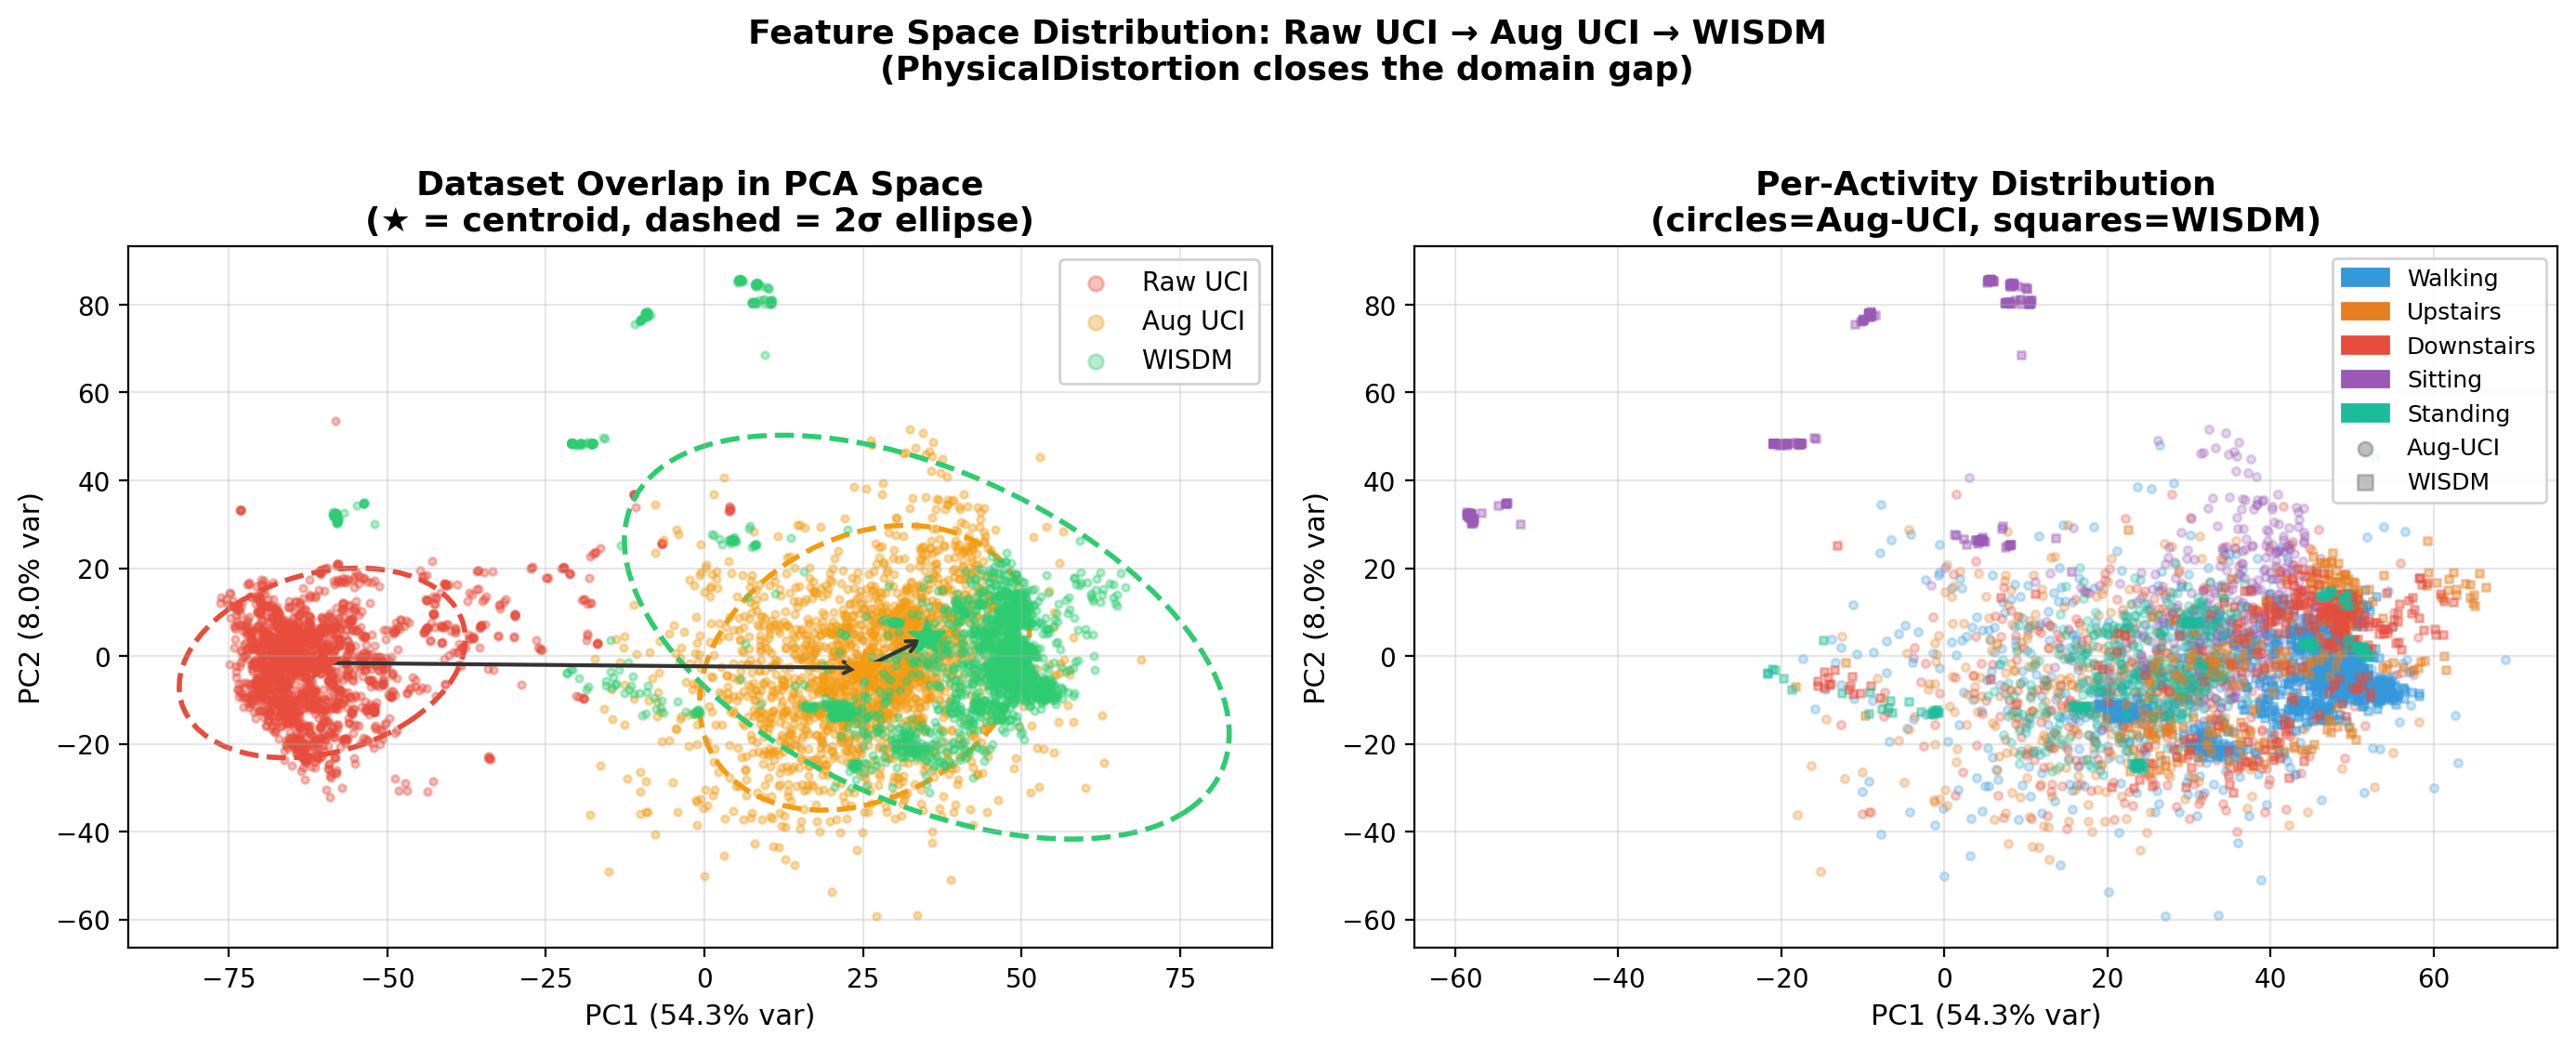
\includegraphics[width=0.85\textwidth]{figures/distribution_alignment.png}
\caption{Distribution alignment before and after PhysicalDistortion. Multi-kernel MMD drops from 0.830 to 0.453 (45.4\% reduction), confirming that the pipeline brings the source distribution closer to the target.}
\label{fig:dist_align}
\end{figure}

Figure~\ref{fig:dist_align} shows the distribution alignment effect quantitatively. The MMD reduction of 45\% is substantial but not complete, which likely explains why performance is still imperfect.

\begin{figure}[htbp]
\centering
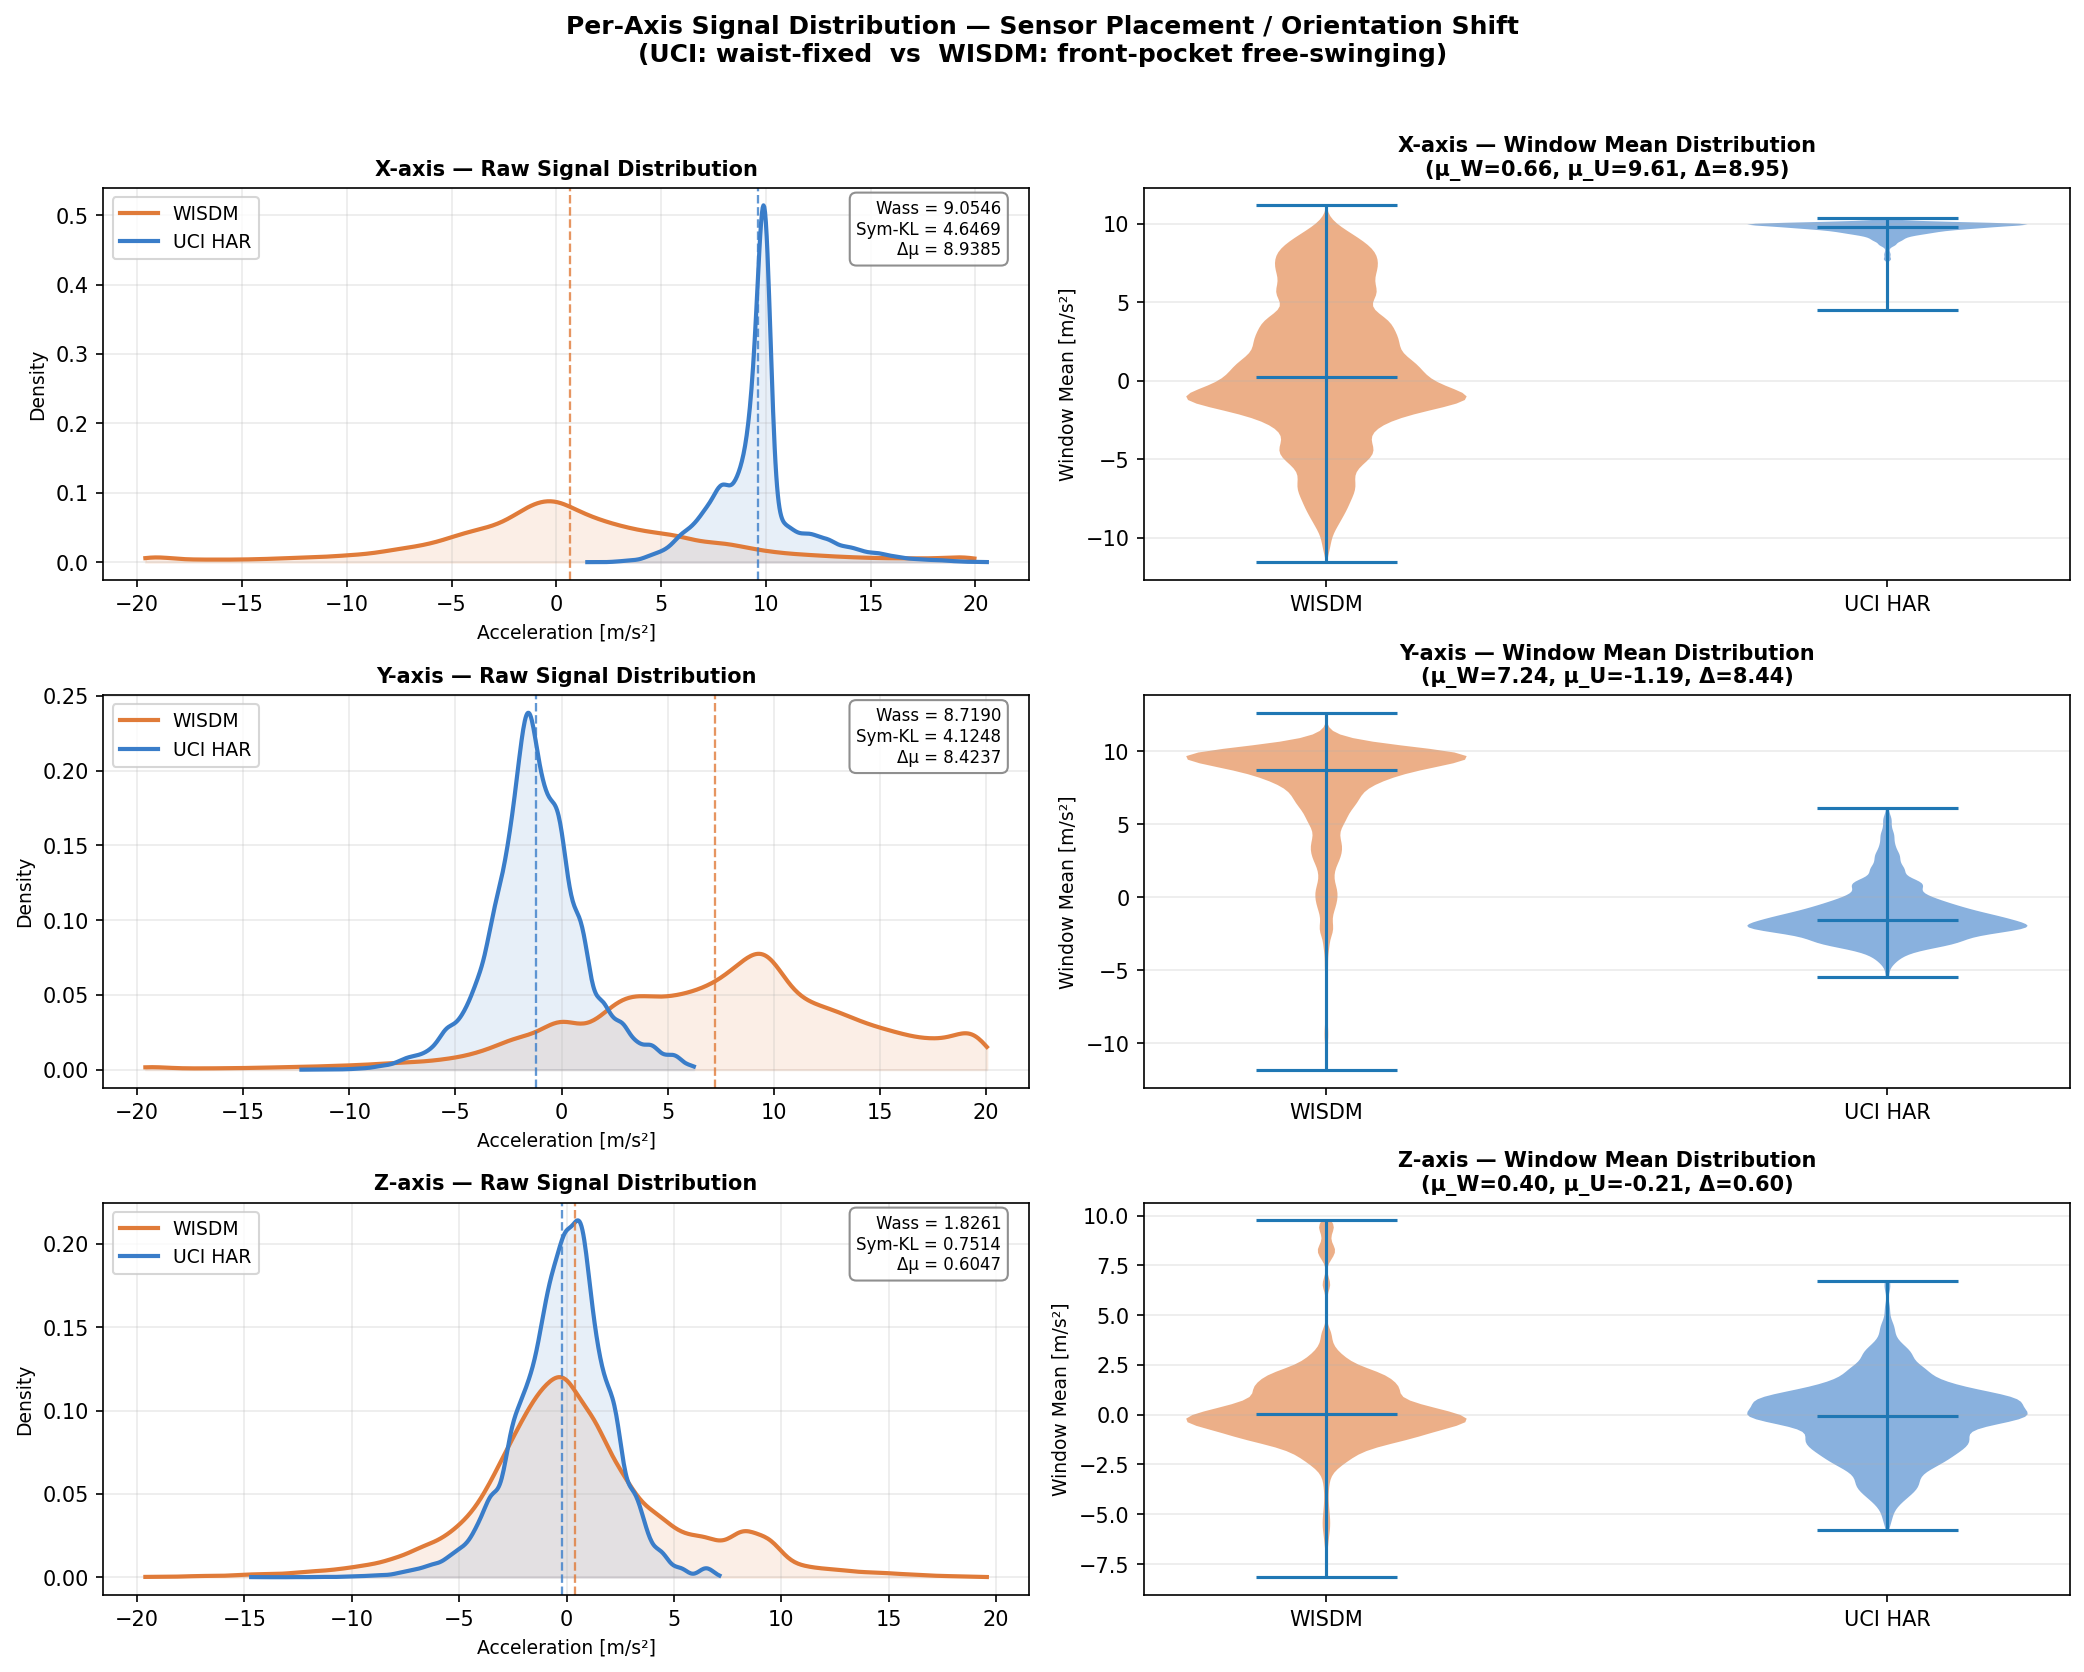
\includegraphics[width=0.85\textwidth]{figures/per_axis_analysis.png}
\caption{Per-axis distribution comparison between UCI HAR and WISDM. The dominant shift is on the X-axis (Wasserstein = 8.7\,m/s$^2$), corresponding to the gravity projection difference between waist-mounted and front-pocket sensors.}
\label{fig:per_axis}
\end{figure}

Figure~\ref{fig:per_axis} shows that the X-axis shift completely dwarfs all other distributional differences. UCI HAR X-axis mean is +8.58\,m/s$^2$ (gravity pointing along X for waist mount), while WISDM Y-axis mean is +6.51\,m/s$^2$ (gravity pointing along Y for front-pocket). The mismatch is both in magnitude and axis.

\subsection{Per-class Performance}

\begin{figure}[htbp]
\centering
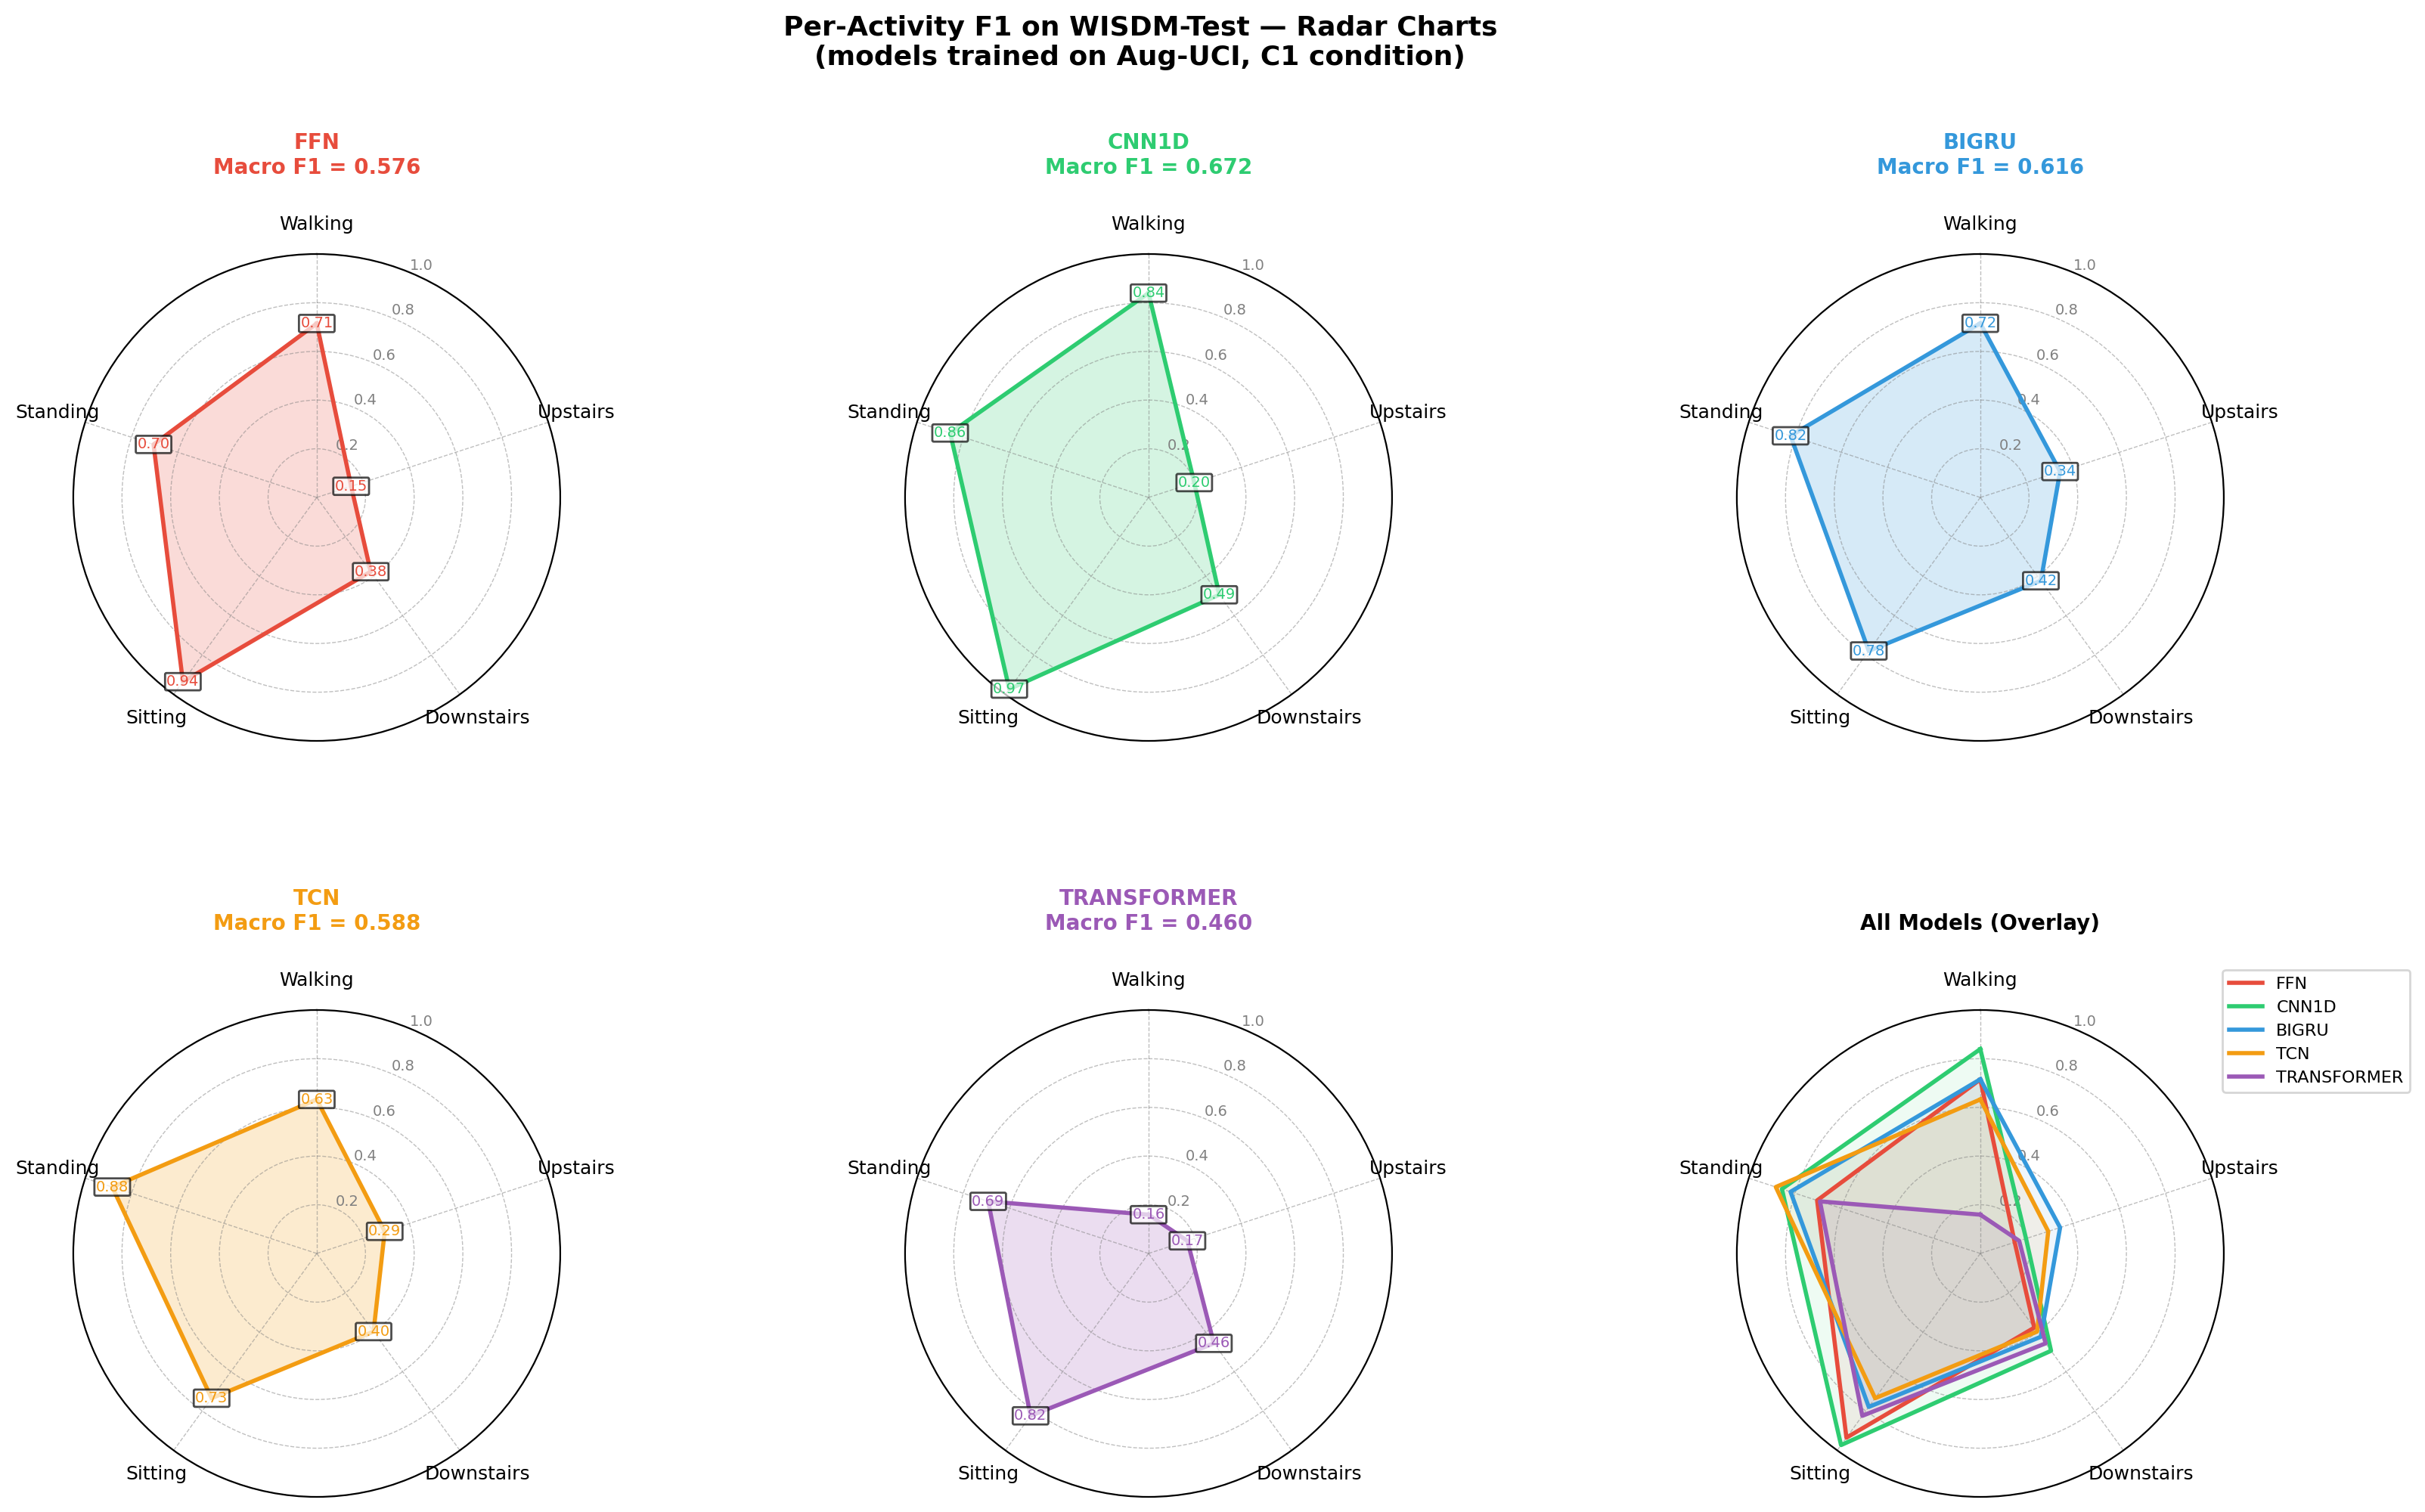
\includegraphics[width=0.75\textwidth]{figures/radar_charts.png}
\caption{Per-class F1 for CNN1D under C1 (PhysicalDistortion). Static activities (Sitting: 0.966, Standing: 0.820) and Walking (0.872) are well-handled. Stair activities remain harder.}
\label{fig:radar}
\end{figure}

Per-class F1 for CNN1D under C1 (Figure~\ref{fig:radar}): Walking 0.872, Upstairs 0.445, Downstairs 0.513, Sitting 0.966, Standing 0.820. The stair activities are clearly the weak point. Sitting and Standing are nearly perfect, probably because their signals are dominated by a static gravity vector that our orientation correction handles well.

\subsection{Hyperparameter Search}

The best CNN1D configuration found by random search (40 trials): channels = (32, 32, 32), 10{,}277 parameters, dropout = 0.39, label smoothing = 0.14, lr = $9 \times 10^{-4}$, weight decay = $4 \times 10^{-3}$, batch size = 128. This achieves F1 = 0.762 on the WISDM test set—an improvement over the default-hyperparameter CNN1D (F1 = 0.723). A larger model did not help; the best configuration is relatively small at 10,277 parameters.

\section{Discussion}

\subsection{Why Data-Level Alignment Works}

The central reason PhysicalDistortion works is that the dominant sources of shift are \emph{physical} rather than semantic. The sensor is mounted differently, samples at a different rate, and has different noise characteristics. None of these differences are about how activities manifest biomechanically—a walking step looks the same in terms of body motion. The domain shift is purely in how that motion is transduced.

When the shift is physical in origin, the right tool is physical correction. PhysicalDistortion addresses this directly: each operator corresponds to a specific, measurable physical difference. The orientation correction handles the gravity axis mismatch (8.7\,m/s$^2$ Wasserstein). The amplitude scaling handles the filter difference. The AR(1) noise handles the temporal correlation structure.

\subsection{Why TTBN and DANN Do Not Help}

Test-time batch normalization assumes that the main distributional mismatch is in feature statistics (mean and variance at each layer). After PhysicalDistortion, the raw input distributions are already much closer, so there is less for TTBN to fix. But TTBN is also harmful here: it uses the test batch to re-estimate statistics, which introduces noise when the batch is small or class-imbalanced (WISDM has Walking at 56\% vs.\ UCI HAR at 20\%, TVD = 0.36). The re-estimated statistics can actually move things in the wrong direction.

DANN hurts even more. The gradient reversal approach works when features exist that are both discriminative for activities and domain-invariant. In our case, the domain shift is tied to the activity itself: stair-climbing in a waist-mounted sensor looks different from stair-climbing in a front-pocket sensor, not because of sensor placement alone, but because the gravity projection changes which axes carry the relevant information. Forcing domain invariance in feature space can destroy that axis-specific information.

There is also a practical issue: DANN requires careful balancing of the domain adversarial loss weight. We tuned this, but the training was unstable and results varied substantially across runs.

\subsection{Honest Evaluation of Remaining Failures}

We should be clear about what the 0.723 F1 does not mean. Upstairs F1 = 0.445 is genuinely bad. Stair climbing at 20\,Hz with a pocket sensor produces a complicated signal with both periodic and aperiodic components, and the inter-subject variation in how people climb stairs is large. Our window-level augmentation operates on fixed-length segments and cannot model the step-to-step variability that differs across subjects.

More generally, inter-subject variability is a real problem we did not solve. The Wasserstein distance across subjects within WISDM reaches 1.891\,m/s$^2$ for some axes, which is non-trivial. Our PhysicalDistortion pipeline is calibrated to the dataset-level mean difference, not to individual subjects. A proper solution would likely require subject-level adaptation, which needs target labels.

The evaluation setup is also limited: hyperparameter selection was guided by macro F1 on WISDM-Val (a held-out WISDM validation split belonging to the target domain). This means the HP-search result of F1 = 0.762 is somewhat optimistic—the selected configuration is tuned toward the target distribution rather than chosen blindly. A truly deployment-blind evaluation would require holding out WISDM entirely from the HP selection process, which we did not do.

\section{Conclusion}

Cross-dataset HAR transfer is hard primarily because the physical sensor setup differs between datasets. We identified seven sources of domain shift between UCI HAR and WISDM~v1.1, with gravity axis projection as the dominant one (Wasserstein = 8.7\,m/s$^2$). Our PhysicalDistortion pipeline, which corrects for these physical differences at the data level, reduces MMD from 0.830 to 0.453 and improves CNN1D F1 from 0.120 to 0.723—without any access to target labels. Adding model-level adaptation (TTBN, DANN) on top of PhysicalDistortion consistently hurts performance, which suggests that physical alignment should be the first step in any cross-dataset HAR transfer pipeline. Remaining gaps, particularly for stair activities, likely require subject-level information that we did not have access to.

\bibliographystyle{plainnat}
\begin{thebibliography}{99}

\bibitem[Ganin et al.(2016)]{ganin2016domain}
Ganin, Y., Ustunova, E., Ajakan, H., Germain, P., Larochelle, H., Laviolette, F., Marchand, M., and Lempitsky, V.
\newblock Domain-adversarial training of neural networks.
\newblock \emph{Journal of Machine Learning Research}, 17(59):1--35, 2016.

\bibitem[Reyes-Ortiz et al.(2016)]{anguita2013public}
Reyes-Ortiz, J., Anguita, D., Ghio, A., Oneto, L., and Parra, X.
\newblock Transition-aware human activity recognition using smartphones.
\newblock \emph{Neurocomputing}, 171:754--767, 2016.

\bibitem[Kwapisz et al.(2011)]{kwapisz2011activity}
Kwapisz, J.~R., Weiss, G.~M., and Moore, S.~A.
\newblock Activity recognition using cell phone accelerometers.
\newblock \emph{ACM SIGKDD Explorations Newsletter}, 12(2):74--82, 2011.

\bibitem[Schneider et al.(2020)]{schneider2020improving}
Schneider, S., Rusak, E., Eck, L., Bringmann, O., Brendel, W., and Bethge, M.
\newblock Improving robustness against common corruptions by covariate shift adaptation.
\newblock \emph{Advances in Neural Information Processing Systems}, 33, 2020.

\bibitem[Wang et al.(2018)]{wang2018stratified}
Wang, J., Chen, Y., Hao, S., Feng, W., and Shen, Z.
\newblock Stratified transfer learning for cross-domain activity recognition.
\newblock In \emph{IEEE International Conference on Pervasive Computing and Communications}, 2018.

\bibitem[Chen et al.(2019)]{chen2019cross}
Chen, K., Zhang, D., Yao, L., Guo, B., Yu, Z., and Liu, Y.
\newblock Deep learning for sensor-based human activity recognition: Overview, challenges, and opportunities.
\newblock \emph{ACM Computing Surveys}, 54(4):1--40, 2021.

\bibitem[Wilson et al.(2020)]{wilson2020multi}
Wilson, G., Doppa, J.~R., and Cook, D.~J.
\newblock Multi-source deep domain adaptation with weak supervision for time-series sensor data.
\newblock In \emph{ACM SIGKDD International Conference on Knowledge Discovery and Data Mining}, 2020.

\bibitem[Um et al.(2017)]{um2017data}
Um, T.~T., Pfister, F.~M.~J., Pichler, D., Endo, S., Lang, M., Hirche, S., Fietzek, U., and Kuli{\'c}, D.
\newblock Data augmentation of wearable sensor data for parkinson's disease monitoring using convolutional neural networks.
\newblock In \emph{International Conference on Multimodal Interaction}, 2017.

\bibitem[Mathur et al.(2021)]{mathur2021unsupervised}
Mathur, A., Lane, N.~D., and Bhatti, S.
\newblock Unsupervised adaptation for deep neural networks in internet of things.
\newblock \emph{Proceedings of the ACM on Interactive, Mobile, Wearable and Ubiquitous Technologies}, 5(2):1--28, 2021.

\bibitem[Sagawa et al.(2019)]{sagawa2019distributionally}
Sagawa, S., Koh, P.~W., Hashimoto, T.~B., and Liang, P.
\newblock Distributionally robust neural networks for group shifts.
\newblock In \emph{International Conference on Learning Representations}, 2020.

\bibitem[Sun and Saenko(2016)]{sun2016deep}
Sun, B. and Saenko, K.
\newblock Deep coral: Correlation alignment for deep domain adaptation.
\newblock In \emph{European Conference on Computer Vision Workshops}, 2016.

\end{thebibliography}

\end{document}
